
%{{第六十三回}}{第六十三回}}

\chapter{寿怡红群芳开夜宴\hspace{.5em}死金丹独艳理亲丧}

{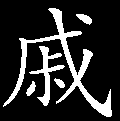
\includegraphics[width=3mm]{../Images/00005} \kaishu 此书写世人之富贵子弟易流邪鄙,其作长上者,有不能稽查之处,如宝玉之夜宴,始见之文雅韵致,细思之,何事生端不基于此?更能写贾蓉之恶赖无耻,亦世家之必有者,读者当以“三人行必有我师”之说为念,方能领会作者之用意也。戒之!}

话说宝玉回至房中洗手,因与袭人商议:“晚间吃酒,大家取乐,不可拘泥。如今吃什么,好早说给他们备办去。”袭人笑道:“你放心,我和晴雯、麝月、秋纹四个人,每人五钱银子,共是二两。芳官、碧痕、小燕、四儿四个人,每人三钱银子,他们有假的不算,共是三两二钱银子,早已交给了柳嫂子,预备四十碟果子。我和平儿说了,已经抬了一坛好绍兴酒藏在那边了。我们八个人单替你过生日。”宝玉听了,喜的忙说:“他们是那里的钱,不该叫他们出才是。”晴雯道:“他们没钱,难道我们是有钱的!这原是各人的心。那怕他偷的呢,只管领他们的情就是。”宝玉听了,笑说:“你说的是。”袭人笑道:“你一天不挨他两句硬话村你,你再过不去。”晴雯笑道:“你如今也学坏了,专会架桥拨火儿。”说着,大家都笑了。宝玉说:“关院门罢。”袭人笑道:“怪不得人说你是‘无事忙’,这会子关了门,人倒疑惑,越性再等一等。”宝玉点头,因说:“我出去走走,四儿舀水去,小燕一个跟我来罢。”说着,走至外边,因见无人,便问五儿之事。小燕道:“我才告诉了柳嫂子,他倒喜欢的很。只是五儿那夜受了委屈烦恼,回家去又气病了,那里来得。只等好了罢。”宝玉听了,不免后悔长叹,因又问:“这事袭人知道不知道?”小燕道:“我没告诉,不知芳官可说了不曾。”宝玉道:“我却没告诉过他,也罢,等我告诉他就是了。”说毕,复走进来,故意洗手。

已是掌灯时分,听得院门前有一群人进来。大家隔窗悄视,果见林之孝家的和几个管事的女人走来,前头一人提着大灯笼。晴雯悄笑道:“他们查上夜的人来了。这一出去,咱们好关门了。”只见怡红院凡上夜的人都迎了出去,林之孝家的看了不少。林之孝家的吩咐:“别耍钱吃酒,放倒头睡到大天亮。我听见是不依的。”众人都笑说:“那里有那样大胆子的人。”林之孝家的又问:“宝二爷睡下了没有?”众人都回不知道。袭人忙推宝玉。宝玉靸了鞋,便迎出来,笑道:“我还没睡呢。妈妈进来歇歇。”又叫:“袭人倒茶来。”林之孝家的忙进来,笑说:“还没睡?如今天长夜短了,该早些睡,明儿起的方早。不然到了明日起迟了,人笑话说不是个读书上学的公子了,倒像那起挑脚汉了。”说毕,又笑。宝玉忙笑道:“妈妈说的是。我每日都睡的早,妈妈每日进来可都是我不知道的,已经睡了。今儿因吃了面怕停住食,所以多顽一会子。”林之孝家的又向袭人等笑说:“该潗些个普洱茶吃。”袭人晴雯二人忙笑说:“潗了一盄子女儿茶,已经吃过两碗了。大娘也尝一碗,都是现成的。”说着,晴雯便倒了一碗来。

林之孝家的又笑道:“这些时我听见二爷嘴里都换了字眼,赶着这几位大姑娘们竟叫起名字来。虽然在这屋里,到底是老太太、太太的人,还该嘴里尊重些才是。若一时半刻偶然叫一声使得,若只管叫起来,怕以后兄弟侄儿照样,便惹人笑话,说这家子的人眼里没有长辈。”宝玉笑道:“妈妈说的是。我原不过是一时半刻的。”袭人晴雯都笑说:“这可别委屈了他。直到如今,他可姐姐没离了口。不过顽的时候叫一声半声名字,若当着人却是和先一样。”林之孝家的笑道:“这才好呢,这才是读书知礼的。越自己谦越尊重,别说是三五代的陈人,现从老太太、太太屋里拨过来的,便是老太太、太太屋里的猫儿狗儿,轻易也伤他不的。这才是受过调教的公子行事。”说毕,吃了茶,便说:“请安歇罢,我们走了。”宝玉还说:“再歇歇。”那林之孝家的已带了众人,又查别处去了。

这里晴雯等忙命关了门,进来笑说:“这位奶奶那里吃了一杯来了,唠三叨四的,又排场了我们一顿去了。”麝月笑道:“他也不是好意的,少不得也要常提着些儿。也堤防着怕走了大褶儿的意思。”说着,一面摆上酒果。袭人道:“不用围桌,咱们把那张花梨圆炕桌子放在炕上坐,又宽绰,又便宜。”说着,大家果然抬来。麝月和四儿那边去搬果子,用两个大茶盘做四五次方搬运了来。两个老婆子蹲在外面火盆上筛酒。宝玉说:“天热,咱们都脱了大衣裳才好。”众人笑道:“你要脱你脱,我们还要轮流安席呢。”宝玉笑道:“这一安就安到五更天了。知道我最怕这些俗套子,在外人跟前不得已的,这会子还怄我就不好了。”众人听了,都说:“依你。”于是先不上坐,且忙着卸妆宽衣。{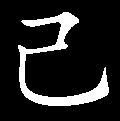
\includegraphics[width=3mm]{../Images/00003}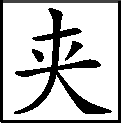
\includegraphics[width=3mm]{../Images/00012}\footnotesize \kaishu 凡吃酒从未先如此者,此独怡红风俗。故王夫人云:“他行事总是与世人两样的”,知子莫过母也。}

一时将正装卸去,头上只随便挽着䰖儿,身上皆是长裙短袄。宝玉只穿着大红棉纱小袄子,下面绿绫弹墨袷裤,散着裤脚,倚着一个各色玫瑰芍药花瓣装的玉色夹纱新枕头,和芳官两个先划拳。当时芳官满口嚷热,{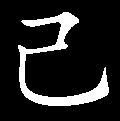
\includegraphics[width=3mm]{../Images/00003}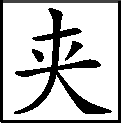
\includegraphics[width=3mm]{../Images/00012}\footnotesize \kaishu 余亦此时太热了,恨不得一冷。既冷时思此热,果然一梦矣。}只穿着一件玉色红青酡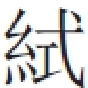
\includegraphics[width=9.4pt,height=9.4pt,align=c,vshift=1pt]{../images/00029}三色缎子斗的水田小夹袄,束着一条柳绿汗巾,底下是水红撒花夹裤,也散着裤腿。头上眉额编着一圈小辫,总归至顶心,结一根鹅卵粗细的总辫,拖在脑后。右耳眼内只塞着米粒大小的一个小玉塞子,左耳上单带着一个白果大小的硬红镶金大坠子,越显的面如满月犹白,眼如秋水还清。引的众人笑说:“他两个倒像是双生的弟兄两个。”袭人等一一的斟了酒来,说:“且等等再划拳,虽不安席,每人在手里吃我们一口罢了。”于是袭人为先,端在唇上吃了一口,馀依次下去,一一吃过,大家方团圆坐定。小燕四儿因炕沿坐不下,便端了两张椅子,近炕放下。那四十个碟子,皆是一色白粉定窑的,不过只有小茶碟大,里面不过是山南海北,中原外国,或干或鲜,或水或陆,天下所有的酒馔果菜。宝玉因说:“咱们也该行个令才好。”袭人道:“斯文些的才好,别大呼小叫,惹人听见。二则我们不识字,可不要那些文的。”麝月笑道:“拿骰子咱们抢红罢。”宝玉道:“没趣,不好。咱们占花名儿好。”晴雯笑道:“正是早已想弄这个顽意儿。”袭人道:“这个顽意虽好,人少了没趣。”小燕笑道:“依我说,咱们竟悄悄的把宝姑娘林姑娘请了来顽一回子,到二更天再睡不迟。”袭人道:“又开门喝户的闹,倘或遇见巡夜的问呢?”宝玉道:“怕什么,咱们三姑娘也吃酒,再请他一声才好。还有琴姑娘。”众人都道:“琴姑娘罢了,他在大奶奶屋里,叨登的大发了。”宝玉道:“怕什么,你们就快请去。”小燕四儿都得不了一声,二人忙命开了门,分头去请。

晴雯、麝月、袭人三人又说:“他两个去请,只怕宝林两个不肯来,须得我们请去,死活拉他来。”于是袭人晴雯忙又命老婆子打个灯笼,二人又去。果然宝钗说夜深了,黛玉说身上不好,他二人再三央求说:“好歹给我们一点体面,略坐坐再来。”探春听了却也欢喜。因想:“不请李纨,倘或被他知道了倒不好。”便命翠墨同了小燕也再三的请了李纨和宝琴二人,会齐,先后都到了怡红院中。袭人又死活拉了香菱来。炕上又并了一张桌子,方坐开了。

宝玉忙说:“林妹妹怕冷,过这边靠板壁坐。”又拿个靠背垫着些。袭人等都端了椅子在炕沿下一陪。黛玉却离桌远远的靠着靠背,因笑向宝钗、李纨、探春等道:“你们日日说人夜聚饮博,今儿我们自己也如此,以后怎么说人。”李纨笑道:“这有何妨。一年之中不过生日节间如此,并无夜夜如此,这倒也不怕。”

说着,晴雯拿了一个竹雕的签筒来,里面装着象牙花名签子,摇了一摇,放在当中。又取过骰子来,盛在盒内,摇了一摇,揭开一看,里面是五点,数至宝钗。宝钗便笑道:“我先抓,不知抓出个什么来。”说着,将筒摇了一摇,伸手掣出一根,大家一看,只见签上画着一支牡丹,题着“艳冠群芳”四字,下面又有镌的小字一句唐诗,道是:

任是无情也动人。

又注着:“在席共贺一杯,此为群芳之冠,随意命人,不拘诗词雅谑,道一则以侑酒。”众人看了,都笑说:“巧的很,你也原配牡丹花。”说着,大家共贺了一杯。宝钗吃过,便笑说:“芳官唱一支我们听罢。”芳官道:“既这样,大家吃门杯好听的。”于是大家吃酒。芳官便唱:

寿筵开处风光好\ldots{}\ldots{}

众人都道:“快打回去。这会子很不用你来上寿,拣你极好的唱来。”芳官只得细细的唱了一支《赏花时》:

翠凤毛翎扎帚叉,闲踏天门扫落花。您看那风起玉尘沙。猛可的那一层云下,抵多少门外即天涯。您再休要剑斩黄龙一线儿差,再休向东老贫穷卖酒家。您与俺眼向云霞。洞宾呵,您得了人可便早些儿回话;若迟呵,错教人留恨碧桃花。

才罢。宝玉却只管拿着那签,口内颠来倒去念“任是无情也动人”,听了这曲子,眼看着芳官不语。湘云忙一手夺了,掷与宝钗。宝钗又掷了一个十六点,数到探春。

探春笑道:“我还不知得个什么呢。”伸手掣了一根出来,自己一瞧,便掷在地下,红了脸,笑道:“这东西不好,不该行这令。这原是外头男人们行的令,许多混话在上头。”众人不解,袭人等忙拾了起来,众人看上面是一枝杏花,那红字写着“瑶池仙品”四字,诗云:

日边红杏倚云栽。

注云:“得此签者,必得贵婿,大家恭贺一杯,共同饮一杯。”众人笑道:“我说是什么呢。这签原是闺阁中取戏的,除了这两三根有这话的,并无杂话,这有何妨。我们家已有了个王妃,难道你也是王妃不成。大喜,大喜。”说着,大家来敬。探春那里肯饮,却被史湘云、香菱、李纨等三四个人强死强活灌了下去。探春只命蠲了这个,再行别的,众人断不肯依。湘云拿着他的手强掷了个十九点出来,便该李氏掣。

李氏摇了一摇,掣出一根来一看,笑道:“好极。你们瞧瞧,这劳什子竟有些意思。”众人瞧那签上,画着一枝老梅,是写着“霜晓寒姿”四字,那一面旧诗是:

竹篱茅舍自甘心。

注云:“自饮一杯,下家掷骰。”李纨笑道:“真有趣,你们掷去罢。我只自吃一杯,不问你们的废与兴。”说着,便吃酒,将骰过与黛玉。黛玉一掷,是个十八点,便该湘云掣。湘云笑着,揎拳掳袖的伸手掣了一根出来。大家看时,一面画着一枝海棠,题着“香梦沉酣”四字,那面诗道是:

只恐夜深花睡去。

黛玉笑道:“‘夜深’两个字,改‘石凉’两个字。”众人便知他趣白日间湘云醉卧的事,都笑了。湘云笑指那自行船与黛玉看,又说:“快坐上那船家去罢,别多话了。”众人都笑了。因看注云:“既云‘香梦沉酣’,掣此签者不便饮酒,只令上下二家各饮一杯。”湘云拍手笑道:“阿弥陀佛,真真好签!”恰好黛玉是上家,宝玉是下家。二人斟了两杯只得要饮。宝玉先饮了半杯,瞅人不见,递与芳官,端起来便一扬脖。黛玉只管和人说话,将酒全折在漱盂内了。湘云便绰起骰子来一掷个九点,数去该麝月。

麝月便掣了一根出来。大家看时,这面上一枝荼縻花,题着“韶华胜极”四字,那边写着一句旧诗,道是:

开到荼縻花事了。

注云:“在席各饮三杯送春。”麝月问怎么讲,宝玉愁眉忙将签藏了说:“咱们且喝酒。”说着,大家吃了三口,以充三杯之数。麝月一掷个十九点,该香菱。香菱便掣了一根并蒂花,题着“联春绕瑞”,那面写着一句诗,道是:

连理枝头花正开。

注云:“共贺掣者三杯,大家陪饮一杯。”香菱便又掷了个六点,该黛玉掣。

黛玉默默的想道:“不知还有什么好的被我掣着方好。”一面伸手取了一根,只见上面画着一枝芙蓉,题着“风露清愁”四字,那面一句旧诗,道是:

莫怨东风当自嗟。

注云:“自饮一杯,牡丹陪饮一杯。”众人笑说:“这个好极。除了他,别人不配作芙蓉。”黛玉也自笑了。于是饮了酒,便掷了个二十点,该着袭人。袭人便伸手取了一支出来,却是一枝桃花,题着“武陵别景”四字,那一面旧诗写着道是:

桃红又是一年春。

注云:“杏花陪一盏,坐中同庚者陪一盏,同辰者陪一盏,同姓者陪一盏。”众人笑道:“这一回热闹有趣。”大家算来,香菱、晴雯、宝钗三人皆与他同庚,黛玉与他同辰,只无同姓者。芳官忙道:“我也姓花,我也陪他一钟。”于是大家斟了酒,黛玉因向探春笑道:“命中该着招贵婿的,你是杏花,快喝了,我们好喝。”探春笑道:“这是个什么,大嫂子顺手给他一下子。”李纨笑道:“人家不得贵婿反挨打,我也不忍的。”说的众人都笑了。

袭人才要掷,只听有人叫门。老婆子忙出去问时,原来是薛姨妈打发人来了,接黛玉的。{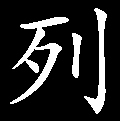
\includegraphics[width=3mm]{../Images/00007}奇文。不接宝钗,而接黛玉。}众人因问几更了,人回:“二更以后了,钟打过十一下了。”宝玉犹不信,要过表来瞧了一瞧,已是子初初刻十分了。黛玉便起身说:“我可撑不住了,回去还要吃药呢。”众人说:“也都该散了。”袭人宝玉等还要留着众人。李纨宝钗等都说:“夜太深了不像,这已是破格了。”袭人道:“既如此,每位再吃一杯再走。”说着,晴雯等已都斟满了酒,每人吃了,都命点灯。袭人等直送过沁芳亭河那边方回来。

关了门,大家复又行起令来。袭人等又用大钟斟了几钟,用盘攒了各样果菜与地下的老嬷嬷们吃。彼此有了三分酒,便猜拳赢唱小曲儿。那天已四更时分,老嬷嬷们一面明吃,一面暗偷,酒坛已罄,众人听了纳罕,方收拾盥漱睡觉。芳官吃的两腮胭脂一般,眉梢眼角越添了许多丰韵,身子图不得,便睡在袭人身上,“好姐姐,心跳的很。”袭人笑道:“谁许你尽力灌起来。”小燕四儿也图不得,早睡了。晴雯还只管叫。宝玉道:“不用叫了,咱们且胡乱歇一歇罢。”自己便枕了那红香枕,身子一歪,便也睡着了。袭人见芳官醉的很,恐闹他唾酒,只得轻轻起来,就将芳官扶在宝玉之侧,由他睡了。自己却在对面榻上倒下。大家黑甜一觉,不知所之。

及至天明,袭人睁眼一看,只见天色晶明,忙说:“可迟了。”向对面床上瞧了一瞧,只见芳官头枕着炕沿上,睡犹未醒,连忙起来叫他。宝玉已翻身醒了,笑道:“可迟了!”因又推芳官起身。那芳官坐起来,犹发怔揉眼睛。袭人笑道:“不害羞,你吃醉了,怎么也不拣地方儿乱挺下了。”芳官听了,瞧了一瞧,方知道和宝玉同榻,忙笑的下地来,说:“我怎么吃的不知道了。”宝玉笑道:“我竟也不知道了。若知道,给你脸上抹些黑墨。”说着,丫头进来伺候梳洗。宝玉笑道:“昨儿有扰,今儿晚上我还席。”袭人笑道:“罢罢罢,今儿可别闹了,再闹就有人说话了。”宝玉道:“怕什么,不过才两次罢了。咱们也算是会吃酒了,那一坛子酒,怎么就吃光了。正是有趣,偏又没了。”袭人笑道:“原要这样才有趣。必至兴尽了,反无后味了。昨儿都好上来了,晴雯连臊也忘了,我记得他还唱了一个。”四儿笑道:“姐姐忘了,连姐姐还唱了一个呢。在席的谁没唱过!”众人听了,俱红了脸,用两手握着笑个不住。

忽见平儿笑嘻嘻的走来,说亲自来请昨日在席的人:“今儿我还东,短一个也使不得。”众人忙让坐吃茶。晴雯笑道:“可惜昨夜没他。”平儿忙问:“你们夜里做什么来?”袭人便说:“告诉不得你。昨儿夜里热闹非常,连往日老太太、太太带着众人顽也不及昨儿这一顽。一坛酒我们都鼓捣光了,一个个吃的把臊都丢了,三不知的又都唱起来。四更多天才横三竖四的打了一个盹儿。”平儿笑道:“好,白和我要了酒来,也不请我,还说着给我听,气我。”晴雯道:“今儿他还席,必来请你的,等着罢。”平儿笑问道:“他是谁,谁是他?”晴雯听了,赶着笑打,说道:“偏你这耳朵尖,听得真。”平儿笑道:“这会子有事不和你说,我干事去了。一回再打发人来请,一个不到,我是打上门来的。”宝玉等忙留,他已经去了。

这里宝玉梳洗了正吃茶,忽然一眼看见砚台底下压着一张纸,因说道:“你们这随便混压东西也不好。”袭人晴雯等忙问:“又怎么了,谁又有了不是了?”宝玉指道:“砚台下是什么?一定又是那位的样子忘记了收的。”晴雯忙启砚拿了出来,却是一张字帖儿,递与宝玉看时,原来是一张粉笺子,上面写着“槛外人妙玉恭肃遥叩芳辰”。{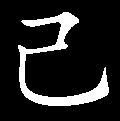
\includegraphics[width=3mm]{../Images/00003}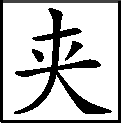
\includegraphics[width=3mm]{../Images/00012}\footnotesize \kaishu 帖文亦蹈俗套之外。}宝玉看毕,直跳了起来,忙问:“这是谁接了来的?也不告诉。”袭人晴雯等见了这般,不知当是那个要紧的人来的帖子,忙一齐问:“昨儿谁接下了一个帖子?”四儿忙飞跑进来,笑说:“昨儿妙玉并没亲来,只打发个妈妈送来。我就搁在那里,谁知一顿酒就忘了。”众人听了,道:“我当谁的,这样大惊小怪。这也不值的。”宝玉忙命:“快拿纸来。”当时拿了纸,研了墨,看他下着“槛外人”三字,自己竟不知回帖上回个什么字样才相敌。只管提笔出神,半天仍没主意。因又想:“若问宝钗去,他必又批评怪诞,不如问黛玉去。”

想罢,袖了帖儿,径来寻黛玉。刚过了沁芳亭,忽见岫烟颤颤巍巍的迎面走来。{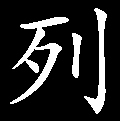
\includegraphics[width=3mm]{../Images/00007}四个俗字写出一个活跳美人,转觉别书中若干“莲步香尘”、“纤腰玉体”字样无味之甚。}宝玉忙问:“姐姐那里去?”岫烟笑道:“我找妙玉说话。”宝玉听了诧异,说道:“他为人孤癖,不合时宜,万人不入他目。原来他推重姐姐,竟知姐姐不是我们一流的俗人。”岫烟笑道:“他也未必真心重我,但我和他做过十年的邻居,只一墙之隔。他在蟠香寺修炼,我家原寒素,赁房居住,就赁的是他庙里的房子,住了十年,无事到他庙里去作伴。我所认的字都是承他所授。我和他又是贫贱之交,又有半师之分。因我们投亲去了,闻得他因不合时宜,权势不容,竟投到这里来。如今又天缘凑合,我们得遇,旧情竟未易。承他青目,更胜当日。”宝玉听了,恍如听了焦雷一般,喜的笑道:“怪道姐姐举止言谈,超然如野鹤闲云,原来有本而来。正因他的一件事我为难,要请教别人去。如今遇见姐姐,真是天缘巧合,求姐姐指教。”说着,便将拜帖取与岫烟看。岫烟笑道:“他这脾气竟不能改,竟是生成这等放诞诡僻了。从来没见拜帖上下别号的,这可是俗语说的‘僧不僧,俗不俗,女不女,男不男’,成个什么道理。”宝玉听说,忙笑道:“姐姐不知道,他原不在这些人中算,他原是世人意外之人。因取我是个些微有知识的,方给我这帖子。我因不知回什么字样才好,竟没了主意,正要去问林妹妹,可巧遇见了姐姐。”

岫烟听了宝玉这话,且只顾用眼上下细细打量了半日,方笑道:“怪道俗语说的‘闻名不如见面’,又怪不得妙玉竟下这帖子给你,又怪不得上年竟给你那些梅花。既连他这样,少不得我告诉你原故。他常说:‘古人中自汉晋五代唐宋以来皆无好诗,只有两句好,说道:纵有千年铁门槛,终须一个土馒头。’所以他自称‘槛外之人’。又常赞文是庄子的好,故又或称为‘畸人’。他若帖子上是自称‘畸人’的,你就还他个‘世人’。畸人者,他自称是畸零之人;你谦自己乃世中扰扰之人,他便喜了。如今他自称‘槛外之人’,是自谓蹈于铁槛之外了;故你如今只下‘槛内人’,便合了他的心了。”宝玉听了,如醍醐灌顶,“嗳哟”了一声,方笑道:“怪道我们家庙说是‘铁槛寺’呢,原来有这一说。姐姐就请,让我去写回帖。”岫烟听了,便自往栊翠庵来。宝玉回房写了帖子,上面只写“槛内人宝玉熏沐谨拜”几字,亲自拿了到栊翠庵,只隔门缝儿投进去便回来了。

因又见芳官梳了头,挽起䰖来,带了些花翠,忙命他改妆,又命将周围的短发剃了去,露出碧青头皮来,当中分大顶,又说:“冬天作大貂鼠卧兔儿带,脚上穿虎头盘云五彩小战靴,或散着裤腿,只用净袜厚底镶鞋。”又说:“芳官之名不好,竟改了男名才别致。”因又改作“雄奴”。芳官十分称心,又说:“既如此,你出门也带我出去。有人问,只说我和茗烟一样的小厮就是了。”宝玉笑道:“到底人看的出来。”芳官笑道:“我说你是无才的。{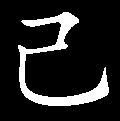
\includegraphics[width=3mm]{../Images/00003}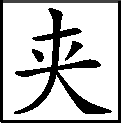
\includegraphics[width=3mm]{../Images/00012}\footnotesize \kaishu 用芳官一骂,有趣。}咱家现有几家土番,你就说我是个小土番儿。况且人人说我打联垂好看,你想这话可妙?”宝玉听了,喜出意外,忙笑道:“这却很好。我亦常见官员人等多有跟从外国献俘之种,图其不畏风霜,鞍马便捷。既这等,再起个番名,叫作‘耶律雄奴’。‘雄奴’二音,又与匈奴相通,都是犬戎名姓。况且这两种人自尧舜时便为中华之患,晋唐诸朝,深受其害。幸得咱们有福,生在当今之世,大舜之正裔,圣虞之功德仁孝,赫赫格天,同天地日月亿兆不朽,所以凡历朝中跳梁猖獗之小丑,到了如今竟不用一干一戈,皆天使其拱手俛头缘远来降。我们正该作践他们,为君父生色。”芳官笑道:“既这样着,你该去操习弓马,学些武艺,挺身出去拿几个反叛来,岂不进忠效力了。何必借我们,你鼓唇摇舌的,自己开心作戏,却说是称功颂德呢。”宝玉笑道:“所以你不明白。如今四海宾服,八方宁静,千载百载不用武备。咱们虽一戏一笑,也该称颂,方不负坐享升平了。”芳官听了有理,二人自为妥贴甚宜。宝玉便叫他“耶律雄奴”。

究竟贾府二宅皆有先人当年所获之囚赐为奴隶,只不过令其饲养马匹,皆不堪大用。湘云素习憨戏异常,他也最喜武扮的,每每自己束銮带、穿折袖,近见宝玉将芳官扮成男子,他便将葵官也扮了个小子。那葵官本是常刮剔短发,好便于面上粉墨油彩,手脚又伶便,打扮了又省一层手。李纨探春见了也爱,便将宝琴的荳官也就命他打扮了一个小童,头上两个丫髻,短袄红鞋,只差了涂脸,便俨是戏上的一个琴童。湘云将“葵官”改了换作“大英”,因他姓韦,便叫他作韦大英,方合自己的意思,暗有“惟大英雄能本色”之语,何必涂朱抹粉,才是男子。荳官身量年纪皆极小,又极鬼灵,故曰荳官。园中人也有唤他作“阿荳”的,也有唤作“炒豆子”的。宝琴反说琴童书童等名太熟了,竟是荳字别致,便换作“荳童”。

因饭后平儿还席,说红香圃太热,便在榆荫堂中摆了几席新酒佳肴。{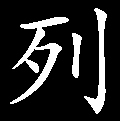
\includegraphics[width=3mm]{../Images/00007}榆荫中者,馀荫也。兹既感灵,今故怀亲,所谓不失忠孝之大纲也。}可喜尤氏又带了配凤\footnote{此侍妾的名字,诸本在本回及第七十四、七十五回均作“佩凤”,在第七十一回则作“配凤”,现统一为“配凤”。}
、偕鸾二妾过来游玩。这二妾亦是青年姣憨女子,不常过来的,今既入了这园,再遇见湘云、香菱、芳、蕊一干女子,所谓“方以类聚,物以群分”二语不错,只见他们说笑不了,也不管尤氏在那里,只凭丫鬟们去伏侍,且同众人一一的游顽。一时到了怡红院,忽听宝玉叫“耶律雄奴”,把配凤、偕鸾、香菱三个人笑在一处,问是什么话,大家也学着叫这名字,又叫错了音韵,或忘了字眼,甚至于叫出“野驴子”来,引的合园中人凡听见者无不笑倒。宝玉又见人人取笑,恐作践了他,忙又说:“海西福朗思牙,闻有金星玻璃宝石,他本国番语以金星玻璃名为‘温都里纳’。如今将你比作他,就改名唤叫‘温都里纳’可好?”芳官听了更喜,说:“就是这样罢。”因此又唤了这名。众人嫌拗口,仍翻汉名,就唤“玻璃”。

闲言少述,且说当下众人都在榆荫堂中以酒为名,大家顽笑,命女先儿击鼓。平儿采了一枝芍药,大家约二十来人传花为令,热闹了一回。因人回说:“甄家有两个女人送东西来了。”探春和李纨尤氏三人出去议事厅相见,这里众人且出来散一散。配凤、偕鸾两个去打秋千顽耍,{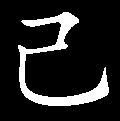
\includegraphics[width=3mm]{../Images/00003}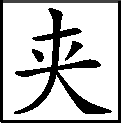
\includegraphics[width=3mm]{../Images/00012}\footnotesize \kaishu 大家千金不令作此戏,故写不及探春等人也。}宝玉便说:“你两个上去,让我送。”慌的配凤说:“罢了,别替我们闹乱子,倒是叫‘野驴子’来送送使得。”宝玉忙笑说:“好姐姐们别顽了,没的叫人跟着你们学着骂他。”偕鸾又说:“笑软了,怎么打呢。掉下来栽出你的黄子来。”配凤便赶着他打。

正顽笑不绝,忽见东府中几个人慌慌张张跑来说:“老爷宾天了。”众人听了,唬了一大跳,忙都说:“好好的并无疾病,怎么就没了?”家下人说:“老爷天天修炼,定是功行圆满,升仙去了。”尤氏一闻此言,又见贾珍父子并贾琏等皆不在家,一时竟没个着己的男子来,未免忙了。只得忙卸了妆饰,命人先到玄真观将所有的道士都锁了起来,等大爷来家审问。一面忙忙坐车带了赖升一干家人媳妇出城。又请太医看视到底系何病。

大夫们见人已死,何处诊脉来,素知贾敬导气之术总属虚诞,更至参星礼斗,守庚申,服灵砂,妄作虚为,过于劳神费力,反因此伤了性命的。如今虽死,肚中坚硬似铁,面皮嘴唇烧的紫绛皱裂。便向媳妇回说:“系玄教中吞金服砂,烧胀而殁。”众道士慌的回说:“原是老爷秘法新制的丹砂吃坏事,小道们也曾劝说‘功行未到且服不得’,不承望老爷于今夜守庚申时悄悄的服了下去,便升仙了。这恐是虔心得道,已出苦海,脱去皮囊,自了去也。”尤氏也不听,只命锁着,等贾珍来发放,且命人去飞马报信。一面看视这里窄狭,不能停放,横竖也不能进城的,忙装裹好了,用软轿抬至铁槛寺来停放。掐指算来,至早也得半月的工夫,贾珍方能来到。目今天气炎热,实不得相待,遂自行主持,命天文生择了日期入殓。寿木已系早年备下寄在此庙的,甚是便宜。三日后便开丧破孝。一面且做起道场来等贾珍。

荣府中凤姐儿出不来,李纨又照顾姊妹,宝玉不识事体,只得将外头之事暂托了几个家中二等管事人。贾?、贾珖、贾珩、贾璎、贾菖、贾菱等各有执事。尤氏不能回家,便将他继母接来在宁府看家。他这继母只得将两个未出嫁的小女带来,一并起居才放心。{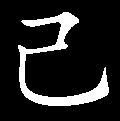
\includegraphics[width=3mm]{../Images/00003}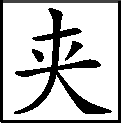
\includegraphics[width=3mm]{../Images/00012}\footnotesize \kaishu 原为放心而来,终是放心而去,妙甚!}

且说贾珍闻了此信,即忙告假,并贾蓉是有职之人。礼部见当今隆敦孝弟,不敢自专,具本请旨。原来天子极是仁孝过天的,且更隆重功臣之裔,一见此本,便诏问贾敬何职。礼部代奏:“系进士出身,祖职已荫其子贾珍。贾敬因年迈多疾,常养静于都城之外玄真观。今因疾殁于寺中,其子珍,其孙蓉,现因国丧随驾在此,故乞假归殓。”天子听了,忙下额外恩旨曰:“贾敬虽白衣无功于国,念彼祖父之功,追赐五品之职。令其子孙扶柩由北下之门进都,入彼私第殡殓。任子孙尽丧礼毕扶柩回籍外,着光禄寺按上例赐祭。朝中由王公以下准其祭吊。钦此。”此旨一下,不但贾府中人谢恩,连朝中所有大臣皆嵩呼称颂不绝。

贾珍父子星夜驰回,半路中又见贾㻞贾珖二人领家丁飞骑而来,看见贾珍,一齐滚鞍下马请安。贾珍忙问:“作什么?”贾㻞回说:“嫂子恐哥哥和侄儿来了,老太太路上无人,叫我们两个来护送老太太的。”贾珍听了,赞称不绝,又问家中如何料理。贾㻞等便将如何拿了道士,如何挪至家庙,怕家内无人接了亲家母和两个姨娘在上房住着。贾蓉当下也下了马,听见两个姨娘来了,便和贾珍一笑。贾珍忙说了几声“妥当”,加鞭便走,店也不投,连夜换马飞驰。一日到了都门,先奔入铁槛寺。那天已是四更天气,坐更的闻知,忙喝起众人来。贾珍下了马,和贾蓉放声大哭,从大门外便跪爬进来,至棺前稽颡泣血,直哭到天亮喉咙都哑了方住。尤氏等都一齐见过。贾珍父子忙按礼换了凶服,在棺前俯伏,无奈自要理事,竟不能目不视物,耳不闻声,少不得减些悲戚,好指挥众人。因将恩旨备述与众亲友听了。一面先打发贾蓉家中料理停灵之事。

贾蓉得不得一声儿,先骑马飞来至家,忙命前厅收桌椅,下槅扇,挂孝幔子,门前起鼓手棚、牌楼等事。又忙着进来看外祖母两个姨娘。原来尤老安人年高喜睡,常歪着,他二姨娘三姨娘都和丫头们作活计,他来了都道烦恼。贾蓉且嘻嘻的望他二姨娘笑说:“二姨娘,你又来了,我们父亲正想你呢。”尤二姐便红了脸,骂道:“蓉小子,我过两日不骂你几句,你就过不得了。越发连个体统都没了。还亏你是大家公子哥儿,每日念书学礼的,越发连那小家子瓢坎的也跟不上。”说着顺手拿起一个熨斗来,搂头就打,吓的贾蓉抱着头滚到怀里告饶。尤三姐便上来撕嘴,又说:“等姐姐来家,咱们告诉他。”

贾蓉忙笑着跪在炕上求饶,他两个又笑了。贾蓉又和二姨抢砂仁吃,尤二姐嚼了一嘴渣子,吐了他一脸。贾蓉用舌头都舔着吃了。众丫头看不过,都笑说:“热孝在身上,老娘才睡了觉,他两个虽小,到底是姨娘家,你太眼里没有奶奶了。回来告诉爷,你吃不了兜着走。”贾蓉撇下他姨娘,便抱着丫头们亲嘴:“我的心肝,你说的是,咱们馋他两个。”丫头们忙推他,恨的骂:“短命鬼儿,你一般有老婆丫头,只和我们闹。知道的说是顽;{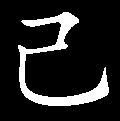
\includegraphics[width=3mm]{../Images/00003}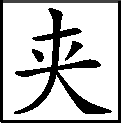
\includegraphics[width=3mm]{../Images/00012}\footnotesize \kaishu 妙极之“顽”,天下有是之顽亦有趣甚,此语余亦亲闻者,非编有也。}不知道的人,再遇见那脏心烂肺的爱多管闲事嚼舌头的人,吵嚷的那府里谁不知道,谁不背地里嚼舌说咱们这边乱账。”贾蓉笑道:“各门另户,谁管谁的事。都够使的了。从古至今,连汉朝和唐朝,人还说脏唐臭汉,何况咱们这宗人家。谁家没风流事,别讨我说出来。连那边大老爷这么利害,琏叔还和那小姨娘不干净呢。凤姑娘那样刚强,瑞叔还想他的账。那一件瞒了我!”

贾蓉只管信口开合胡言乱道之间,只见他老娘醒了,请安问好,又说:“难为老祖宗劳心,又难为两位姨娘受委屈,我们爷儿们感戴不尽。惟有等事完了,我们合家大小,登门去磕头。”尤老安人点头道:“我的儿,倒是你们会说话。亲戚们原是该的。”又问:“你父亲好?几时得了信赶到的?”贾蓉笑道:“才刚赶到的,先打发我瞧你老人家来了。好歹求你老人家事完了再去。”说着,又和他二姨挤眼,那尤二姐便悄悄咬牙含笑骂:“很会嚼舌头的猴儿崽子,留下我们给你爹作娘不成!”贾蓉又戏他老娘道:“放心罢,我父亲每日为两位姨娘操心,要寻两个又有根基又富贵又年青又俏皮的两位姨爹,好聘嫁这二位姨娘的。这几年总没拣得,可巧前日路上才相准了一个。”尤老只当真话,忙问是谁家的,二姊妹丢了活计,一头笑,一头赶着打。说:“妈别信这雷打的。”连丫头们都说:“天老爷有眼,仔细雷要紧!”又值人来回话:“事已完了,请哥儿出去看了,回爷的话去。”那贾蓉方笑嘻嘻的去了。不知如何,且听下回分解。

{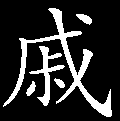
\includegraphics[width=3mm]{../Images/00005} \kaishu 总评:宝玉品高性雅,其终日花围翠绕,用力维持其间,淫荡之至,而能使旁人不觉,被人不厌。贾蓉不分长幼微贱,纵意驰骋于中,恶习可恨。二人之形景天渊,而终归于邪,其滥一也,所谓五十步之间耳。持家有意于子弟者,揣此以照察之可也!}
